\subsubsection{Experimento 1: Efecto de la variaci\'on de colores}
\par Para empezar con la experimentaci\'on relacionada a los tiempos de ejecuci\'on de los distintos m\'etodos correremos los distintos m\'etodos sobre un video con colores constantes y otro video con colores variables y compararemos los resultados obtenidos. Esto nos va a servir a la hora de llevar a cabo otros experimentos, porque si los tiempos son similares entre un video y otro significa que los colores que elijamos para los distintos videos no van a influirnos en los tiempos de ejecuci\'on.

\par Vamos a crear un video que tiene resoluci\'on de 10px x 10px con un color fijo constante y otro video, de la misma resoluci\'on, pero con colores que oscilan de forma ordenada entre el blanco, el negro y sus tonos intermedios. Tomaremos bloques de 5 frames (podr\'iamos haber elegido cualquier n\'umero) y agregaremos 2 frames intermedios entre cada frame del video de entrada.


\subsubsubsection{Resultados del experimento 1}

\begin{figure}[ht]
	\begin{center}
		\subfigure [M\'etodo del Vecino mas cercano] {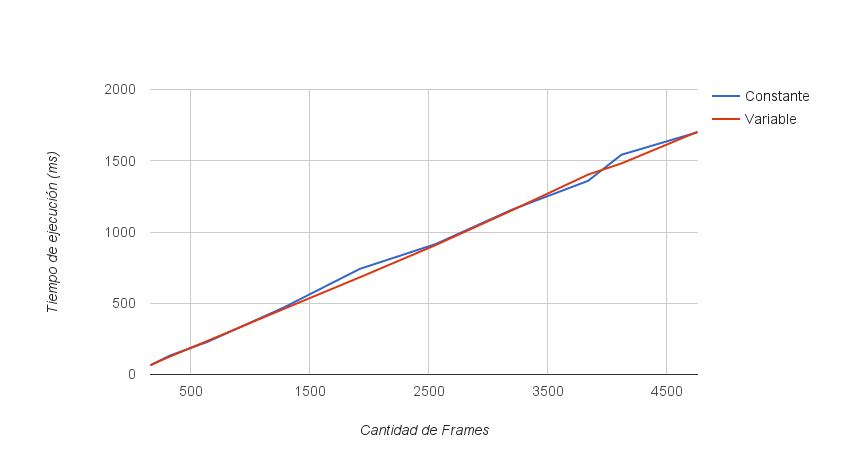
\includegraphics[width=0.70\columnwidth]{imagenes/tiempos/graf1_0.png}}
		\subfigure [M\'etodo Lineal] {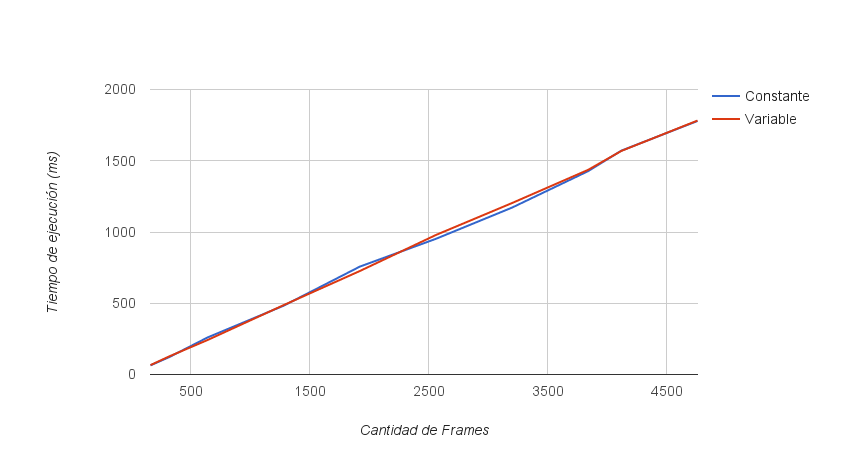
\includegraphics[width=0.49\columnwidth]{imagenes/tiempos/graf1_1.png}}
		\subfigure [M\'etodo de Splines naturales por bloques] {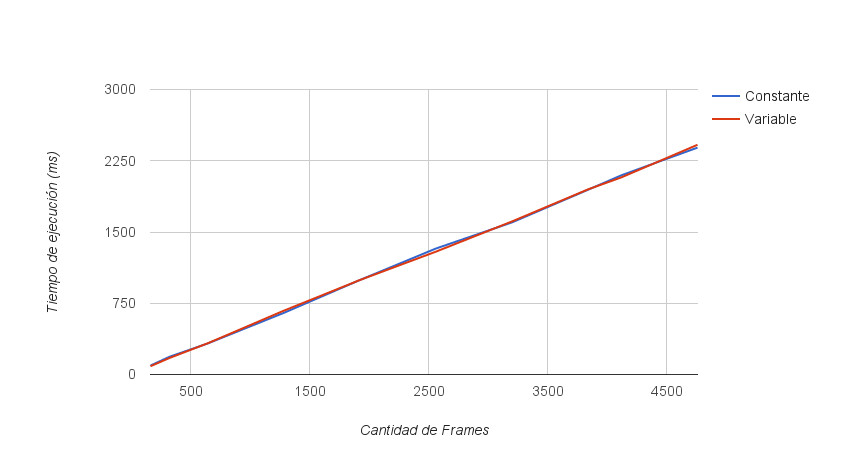
\includegraphics[width=0.49\columnwidth]{imagenes/tiempos/graf1_2.png}}
	\end{center}
\end{figure}


\par Como podemos observar en los gr\'aficos, los m\'etodos se comportan de la misma forma con ambas im\'agenes. Se notan diferencias en algunos momentos del m\'etodo del vecino mas cercano, pero manteniendo el mismo orden. No nos van a preocupar mucho estas diferencias, pero si las tendremos en cuenta de aqu\'i en adelante.
\par Luego de este experimento podemos asumir que el cambio de colores pr\'acticamente no va a influir en los tiempos de ejecuci\'on. Ahora s\'i' podemos continuar con la experimentaci\'on teniendo en claro que ocurre con los colores.


\subsubsection{Experimento 2: Tiempos de ejecucí\'on vs Cantidad de Frames}
\par En este experimento vamos a comparar el tiempo de ejecuci\'on de los diferentes m\'etodos al aumentar la cantidad de frames de un video y tratar de determinar el orden de los mismos. Esper\'abamos que el orden del m\'etodo de Splines por bloques sea mayor, pero eniendo en cuenta lo visto en el Experimento 1 estamos mas cerca de creer que se comportan de forma lineal. Igualmente queremos llevar a cabo este experimento para abarcar cantidades mayores y sacarnos las dudas.

\par Para llevar a cabo el experimento vamos a crear videos con patrones de im\'agenes repetidos (tomando en consideraci\'on esos pequeños cambios que vimos en el experimento anterior) manteniendo el mismo ancho y alto de im\'agenes y cantidad de frames en aumento. Correremos los m\'etodos con un valor de frames intermedios fijo para enfocarnos solo en la cantidad de frames.


\subsubsubsection{Resultados del experimento 2}
\begin{figure}[ht]
	\begin{center}
		\subfigure [Tiempos de ejecuci\'on variando la cantidad de frames] {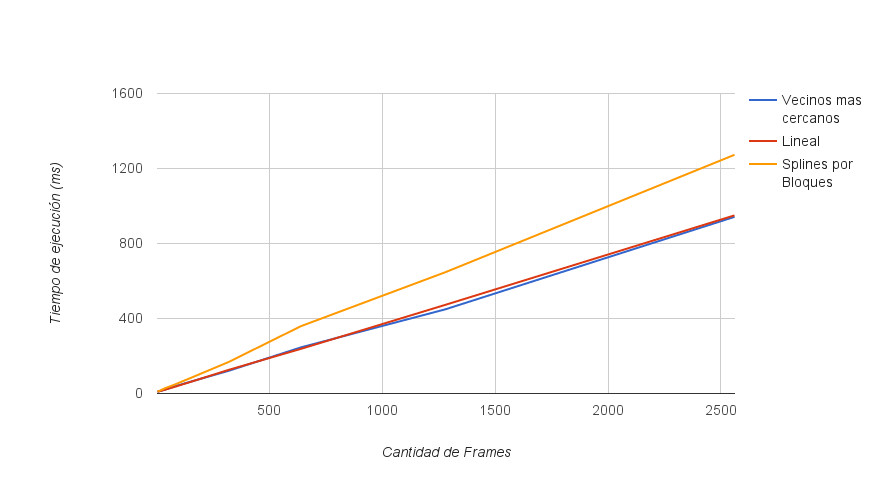
\includegraphics[width=0.9\columnwidth]{imagenes/tiempos/graf2.png}}
	\end{center}
\end{figure}
\par Luego de realizar el experimento podemos creer que el tiempo de ejecuci\'on de los tres m\'etodos es de orden lineal. Podemos notar que los Splines por Bloques se mantiene siempre por encima de los otros, pero mantienen su forma lineal. Mas adelante veremos las diferencias de calidad entre los m\'etodos y tendremos que tener en cuenta esta igualdad de orden, ya que no es tan grande como esper\'abamos en un principio. 





\subsubsection{Experimento 3: Tiempos de ejecucí\'on vs Tama\~no de Bloques}
\par Como tomamos la determinación de aplicar el m\'etodo de Splines de a bloques de frames, queremos medir cuanto nos afecta el tama\~no que decidamos darle a estos bloques en el tiempo de ejecuci\'on del m\'etodo.

\par Para esto vamos a tomar un video con 20480 frames, y vamos a comenzar a aumentar el tama\~no de los bloques hasta llegar a un solo bloque que abarque todos el video.


\subsubsubsection{Resultados del experimento 3}
\begin{figure}[ht]
	\begin{center}
		\subfigure [Tiempos de ejecuci\'on variando el tamaño de los bloques] {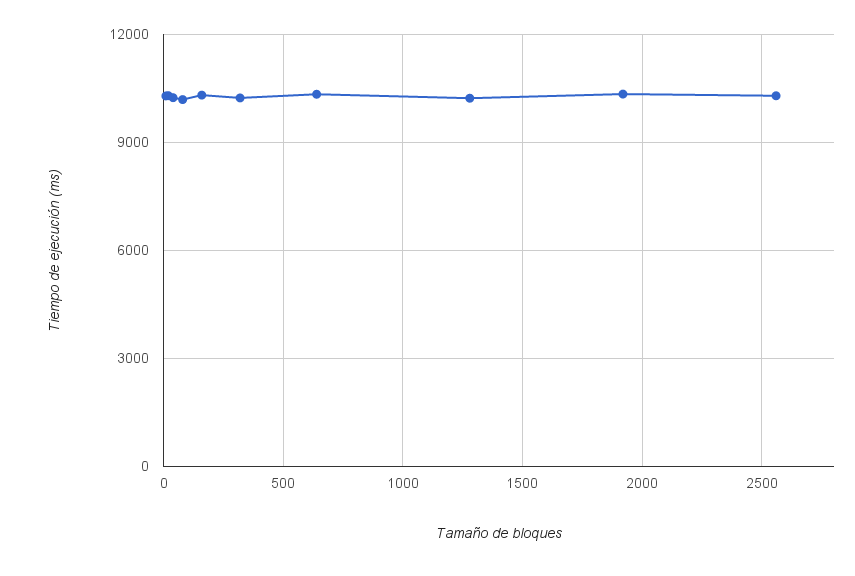
\includegraphics[width=0.9\columnwidth]{imagenes/tiempos/graf3.png}}
	\end{center}
\end{figure}
\par Podemos observar que a pesar de algunas diferencias el orden del tiempo se mantiene constante y no se vi\'o afectado por el aumento del tama\~no de bloques. Nos parece normal que esto ocurra, ya que el algoritmo realiza la misma cantidad de pasos. La diferencia se ve en como se agrupan los datos, lo que si puede influir en las im\'agenes decididas a agregar como nuevos frames.



\subsubsection{Experimento 4: Tiempos de ejecucí\'on vs Cantidad de frames intermedios}
\par Vamos a observar como se comportan los m\'etodos al variar la cantidad de frames que se desean agregar. A pesar de que no se hacen muchos pasos extra para agregar un frame intermedio y solo se realiza una ecuaci\'on, esta ecuaci\'on se repite para cada pixel del nuevo frame. Creemos que esto va a afectar mucho en el tiempo de ejecuci\'on de los tres m\'etodos.

\subsubsubsection{Resultados del experimento 4}
\begin{figure}[ht]
	\begin{center}
		\subfigure [Tiempos de ejecuci\'on variando la cantidad de frames intermedios] {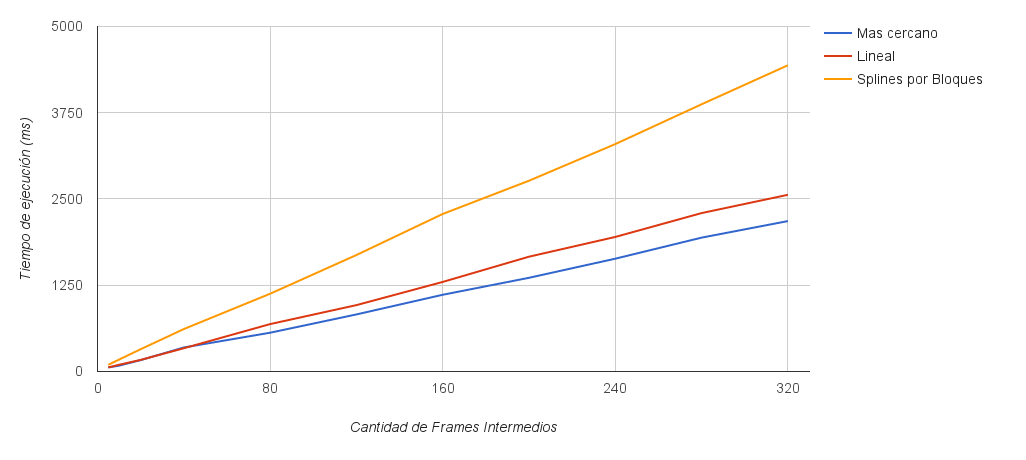
\includegraphics[width=0.9\columnwidth]{imagenes/tiempos/graf4.png}}
	\end{center}
\end{figure}
\par Tras realizar el experimento notamos que el aumento de la cantidad de frames intermedios se relaciona de forma lineal con el tiempo de ejecuci\'on. Analicemos un poco mas la situaci\'on:

\par Supangamos que tomamos N como la cantidad de frames del video original y F como cantidad de frames intermedios a agregar. De esta forma al aplicar alguno de los m\'etodos se agregan F frames N-1 veces $\longrightarrow$ F*(N-1). Si aplicamos uno de los m\'etodo nuevamente, pero esta vez con F+1 frames intermedios, se agregar\'an F+1 frames N-1 veces $\longrightarrow$ (F+1)*(N-1) = F*(N-1) + (N-1). Con este razonamiento simple y sin entrar en detalles podemos convencernos de que al aumentar la cantidad de frames aumentamos de forma lineal la cantidad de operaciones a realizar (agregamos N-1 operaciones `agregar frame intermedio').